\section{REST para consultar: Revisión Técnica Vehicular}
\begin{frame}{Consulta de turnos del RTV}
\tema{Kevin García · REST para consultar}
\begin{columns}[T,onlytextwidth]
\begin{column}{.56\textwidth}
{\Large El solicitante consulta\par el estado de su turno.}\par\medskip
El RTV gestiona turnos, pagos e inspecciones. El personal trabaja desde una web conectada al backend.
\end{column}
\begin{column}{.37\textwidth}
{\color{acento}\bfseries Cliente externo}\par\smallskip
Acceso a un turno propio.\par\medskip
{\color{acento}\bfseries GET}\par\smallskip
Consulta sin modificar el turno.
\end{column}
\end{columns}
\vspace{6mm}
{\color{borde}\hrule}\medskip
\kgnota{Prueba: una cuenta ficticia vinculada a un propietario y a su turno.}
\note{40 segundos. Explicar el sistema y quién lo utiliza. La operación es consultar, no registrar. El entorno de prueba utiliza una cuenta ficticia; no representa una medición de carga real.}
\end{frame}

\begin{frame}[plain]
\centering
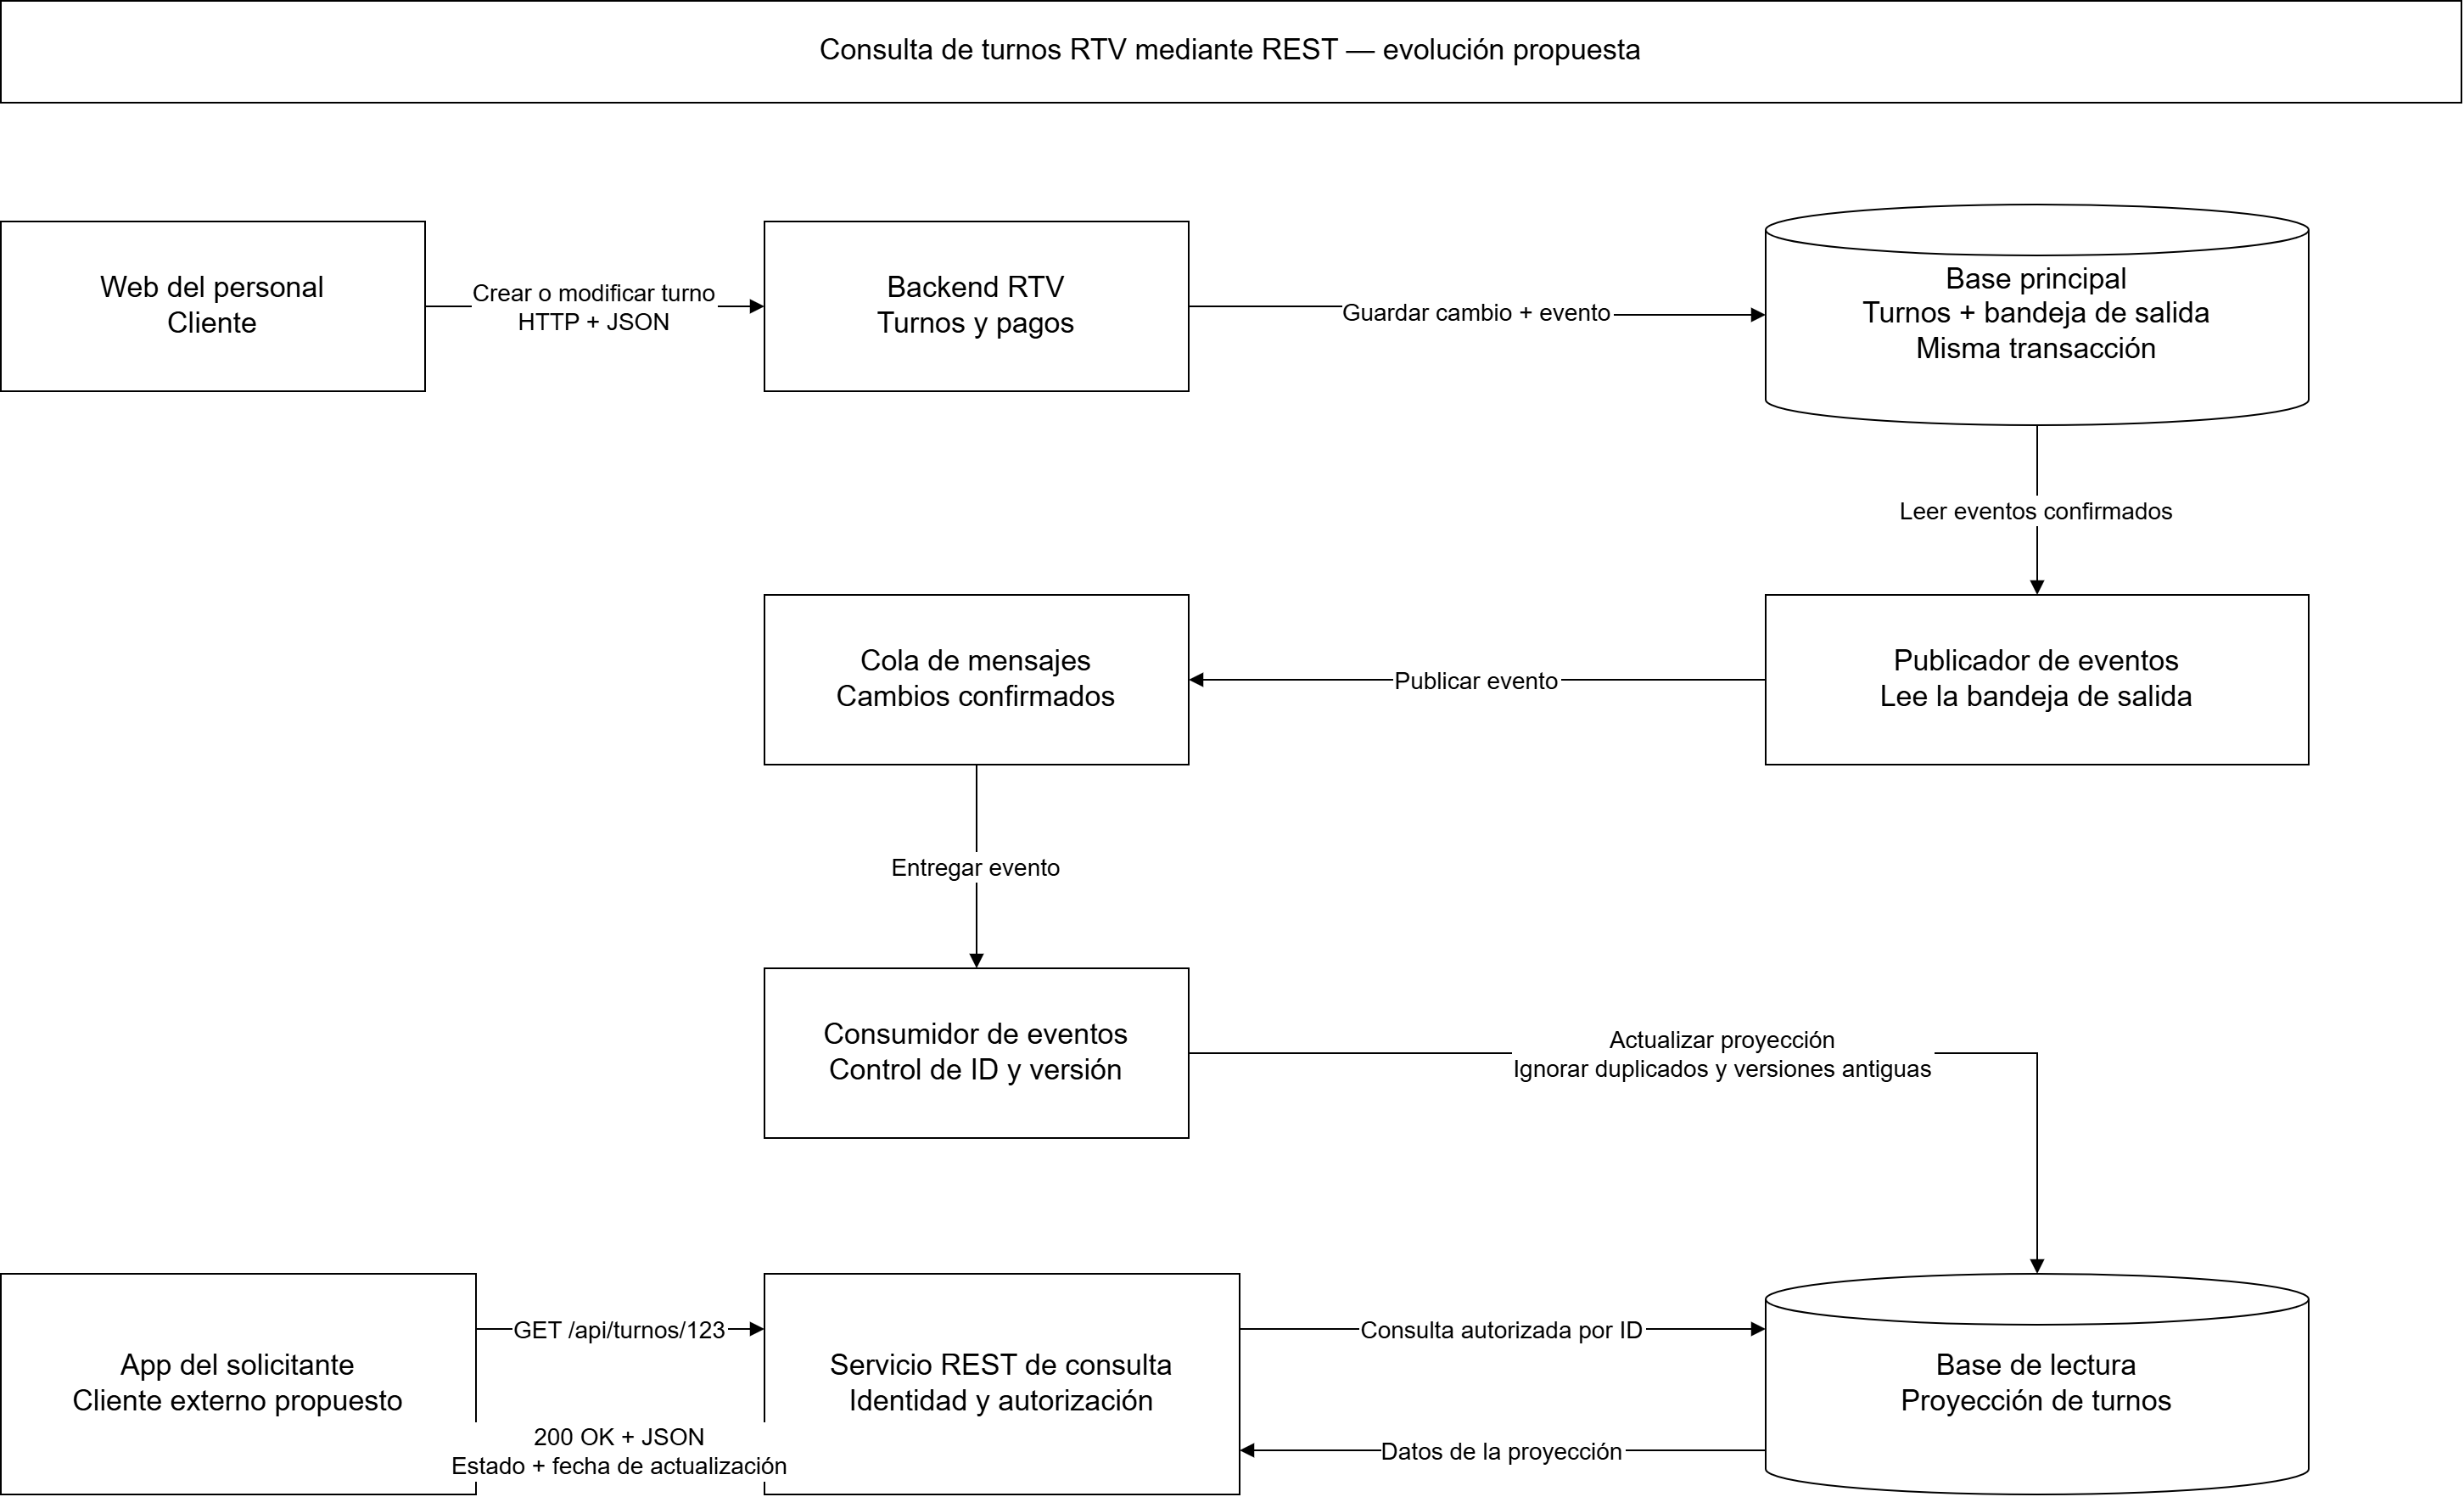
\includegraphics[width=\textwidth,height=.94\paperheight,keepaspectratio]{../diagramas/kevin-rest.png}
\note{Arquitectura de consulta propuesta. Seguir las flechas del diagrama de draw.io. La cola, el consumidor y la base de lectura independiente corresponden a una evolución futura. La demo actual utiliza GET /api/consulta/turnos/82; el identificador 123 del diagrama es ilustrativo.}
\end{frame}

\begin{frame}[fragile]{Consulta probada en el RTV}
\tema{GET /api/consulta/turnos/82}
\begin{columns}[T,onlytextwidth]
\begin{column}{.51\textwidth}
{\color{acento}\Large\bfseries 200 OK}\par
\begin{verbatim}
{
  "turnoId": 82,
  "estado": "GENERADO",
  "fechaInicio": "2026-11-20",
  "fechaFin": null
}
\end{verbatim}
\end{column}
\begin{column}{.43\textwidth}
\textbf{Solo el turno del solicitante}\par\medskip
El backend comprueba el vínculo entre usuario, propietario y turno.\par\medskip
\begin{tabular}{@{}ll@{}}
\textcolor{acento}{\bfseries 404} & Turno ajeno o inexistente\\[2mm]
\textcolor{acento}{\bfseries 401} & Sin sesión\\[2mm]
\textcolor{acento}{\bfseries 403} & Ruta interna del personal
\end{tabular}
\end{column}
\end{columns}
\vspace{2mm}
\kgnota{Cliente externo + Spring Boot + PostgreSQL. Las fechas del JSON corresponden al turno.}
\note{50 segundos. Mostrar 200 para el turno propio 82 y 404 para el turno ajeno 22. La identidad se obtiene de la sesión: el cliente no elige al propietario. El 403 corresponde al solicitante que intenta entrar a una ruta del personal. La ruta /api/turnos/123 del diagrama original es ilustrativa.}
\end{frame}

\begin{frame}{Consistencia y manejo de fallos}
\begin{columns}[T,onlytextwidth]
\begin{column}{.47\textwidth}
\tema{Durante una partición · CAP}
La lectura podría continuar con datos anteriores si se interrumpe la propagación.\par\medskip
La inspección esperaría si no puede confirmar el pago vigente.
\end{column}
\begin{column}{.47\textwidth}
\tema{Sin partición · PACELC}
Se aceptaría retraso de la lectura para evitar esperar cada actualización de la base principal.\par\medskip
Si la API falla: informar y permitir reintentar.
\end{column}
\end{columns}
\vspace{5mm}
{\color{borde}\hrule}\medskip
\kgnota{REST requiere definir peticiones y respuestas~\cite[sec.~3.2.1]{lercher_microservice_2024}. SOAP se consideraría si la integración exigiera WSDL.}
\note{35 segundos. CAP y PACELC describen la arquitectura propuesta, no propiedades de REST. Continuar leyendo supone que el servicio y su base siguen accesibles. Para confirmar pagos se usa la información vigente del servicio responsable. Un resultado anterior se identifica con su fecha. No afirmar que REST es siempre más rápido que SOAP.}
\end{frame}

